% \chapter{Issues with evaluation of distributional models}
% \label{cha:reflection}

% \section{Limitations of current similarity datasets}
% \label{sec:notion-similarity}

% In contrast to linguistic datasets which contain randomly paired words from a broad selection, datasets that come from psychology contain entries that belong to a single category such as \textit{verbs of judging} \cite{FILLENBAUM197454} or \textit{animal terms} \cite{HENLEY1969176}. The reason for category oriented similarity studies is that ``stimuli can only be compared in so far as they have already been categorised as identical, alike, or equivalent at some higher level of abstraction'' \cite{turner1987rediscovering}. Moreover, because of the \emph{extension effect} \cite{medin1993respects}, the similarity of two entries in a context is less than the similarity between the same entries when the context is extended. ``For example, \textit{black} and \textit{white} received a similarity rating of 2.2 when presented by themselves; this rating increased to 4.0 when \textit{black} was simultaneously compared with \textit{white} and \textit{red} (\textit{red} only increased 4.2 to 4.9)'' \cite{medin1993respects}. In the first case \textit{black} and \textit{white} are more dissimilar because they are located on the extremes of the greyscale, but in the presence of \textit{red} they become more similar because they are both monochromes.

% Both MEN and SimLex-999 provide pairs that do not share any similarity to control for false positives, and they do not control for the comparison scale. This makes similarity judgements ambiguous as it is not clear what low similarity values mean: incompatible notions or contrast in meaning. SimLex-999 assigns low similarity scores to the incompatible pairs (0.48, \textit{trick} and \textit{size}) and to antonymy (0.55, \textit{smart} and \textit{dumb}), but \textit{smart} and \textit{dumb} have relatively much more in common than \textit{trick} and \textit{size}!

\chapter{PhraseRel: an IR-inspired compositional dataset}
\label{sec:phraserel}

Datasets that quantify relationships between words have a long history. Some of the most well-known datasets are RG65 \cite{Rubenstein:1965:CCS:365628.365657}, WordSim \cite{2002:PSC:503104.503110}, BLESS \cite{baroni-lenci:2011:GEMS}, MEN \cite{Bruni:2014:MDS:2655713.2655714} and SimLex-999 \cite{hill2014simlex}. All of them have been applied to evaluate the distributional models of meaning.

Naturally, the idea of capturing lexical relationships was extended to phrases and sentences. Many phrase and sentence datasets exist, such as the MS Paraphrase Corpus \cite{dolan2005par} or the phrase entailment dataset of \newcite{baroni-EtAl:2012:EACL2012}. These are potentially applicable to evaluating compositional distributional models of meaning. We say potentially because the grammar-preserving compositional settings \cite{baroni2014frege,DBLP:journals/corr/abs-1003-4394}  rely on high dimensional tensor spaces which do not, at the moment, scale up to  the complex syntactic structures of such datasets. Instead, a family of phrasal, mostly \emph{similarity}-oriented datasets \cite{mitchell-lapata:2008:ACLMain,Grefenstette:2011:ESC:2145432.2145580,kartsaklis-sadrzadeh:2013:EMNLP,kartsadrqpl2014} are widely used for the evaluation of these models \cite{milajevs-EtAl:2014:EMNLP2014,kim-demarneffe-foslerlussier:2015:VSM-NLP}.

We extend the possibility of evaluating compositional distributional models by proposing a task and a corresponding dataset  with controlled syntax. The task focuses on \emph{relevance}, a notion from Information Retrieval (IR).  Further, this task will assist with the understanding of how compositional distributional  models  can be used in IR, without limiting the choice of compositional methods. Much of the original research in distributional semantics has stemmed from vector models of IR, but the IR-NLP connection has been less apparent in  the newer compositional distributional models; our work attempts to bring them back together.

\newcite{Milajevs:2015:IMN:2808194.2809448} got promising results when testing distributional methods in an IR-inspired setting, improving over an IR baseline. However, that work was based on a \emph{similarity} gold standard with a tweaked evaluation method.

To overcome that flaw, we introduce a dataset that measures relevance. To develop the dataset, we took the  dataset of \newcite{kartsaklis-sadrzadeh:2013:EMNLP,kartsadrqpl2014} as the base, extensively extended it with query-document phrase pairs and re-annotated it using Amazon Mechanical Turk, asking for relevance judgements.

The dataset and all referred data files are available at \url{\BASEURL}.

\section{Preparation of candidate entries for the dataset}
\label{sec:design}

As the base, we took the 72 unique sentences from the dataset of \newcite{kartsaklis-sadrzadeh:2013:EMNLP,kartsadrqpl2014}, which is later referred to as \emnlp/.\footnotemark{} These sentences formed the candidate \emph{query sentences}. We paired each query sentence with 23 \emph{document sentences} obtained by four conceptually different methods. Note that even though similarity is different from relevance, it has been used in the IR setting---see for example \newcite{2016arXiv160801972K}.
%
\footnotetext{\url{http://compling.eecs.qmul.ac.uk/wp-content/uploads/2015/07/KS2014.txt}}

\begin{figure*}
  \centering
  \tiny
  \begin{tabular}{lllllllllll}
    \toprule
    \multicolumn{3}{c}{Query} &
    \multicolumn{3}{c}{Document} &
    \multirow{2}{*}{Method} &
    \multicolumn{3}{c}{Relevance} &
    \multirow{2}{*}{Diverse}
    % \multirow{2}{*}{Diverse query}
    \\
    \cmidrule(r){1-3} \cmidrule(r){4-6} \cmidrule(r){8-10}
    Subject  & Verb & Object   & Subject  & Verb   & Object & &
    Mean & Std. & Type & \\
    \midrule
    delegate & buy  & land     & agent    & sell      & property & ks14 &
    1.33 & 1.53 & strict & false  \\
    agent & sell & property &
    delegate       & buy       & land       & ks14       &
    2.00  & 1.00 & strict & false \\

    agent & sell & property &
    representative & exchange  & possession & wordnet:hyper &
    1.00  & 1.73 & N/A & false    \\


    agent & sell & property &
    deputy         & trade     & estate     & wordnet:hypo  &
    1.00  & 0.00 & loose & false  \\

    agent & sell & property &
    people         & buy       & home       & frequency:0   &
    1.33  & 1.53 & strict & false \\

    agent & sell & property &
    company        & offer     & product    & frequency:1   &
    -2.00 & 1.73 & N/A & false    \\

    agent & sell & property &
    people         & advertise & product    & frequency:2   &
    -2.00 & 1.00 & N/A & false    \\

    agent & sell & property &
    family         & buy       & home       & selection     &
    -1.33 & 1.53 & N/A & false    \\

    agent & sell & property &
    company        & specify   & need       & selection     &
    -3.00 & 0.00 & N/A & false    \\

    agent & sell & property &
    people         & represent & set        & selection     &
    -3.00 & 0.00 & N/A & false    \\

    student & acquire & skill &
    student        & gain      & experience & selection     &
    2.00    & 1.00 & strict & true \\
  \bottomrule
  \end{tabular}
  \caption{An Example of query-document pairs}
  \label{fig:emnlp-pairing}
\end{figure*}


%%% Local Variables:
%%% mode: latex
%%% TeX-master: "../thesis"
%%% End:


\subsection{Entries taken from the \emnlp/ datasets}

Each query sentence is paired with a counterpart sentence from the high similarity band\footnotemark{} in the \emnlp/ dataset by treating the similarity band assignments as symmetric. For example, given a \emnlp/ combination
%
\footnotetext{%
The \emnlp/ dataset consists of three bands of intended similarity:
\begin{compactitem}
\item high similarity \dataurl{emnlp2013_turk_HighSim.txt},
\item medium similarity \dataurl{emnlp2013_turk_MedSim.txt},
\item low similarity \dataurl{emnlp2013_turk_LowSim.txt}.
\end{compactitem}
}
%
\begin{eqnarray*}
(\textmd{agent}, \textmd{sell}, \textmd{property}),
(\textmd{delegate}, \textmd{buy}, \textmd{land})
\end{eqnarray*}
%
in the high similarity band, we generated two query-document permutations listed
in Figure~\ref{fig:emnlp-pairing} with the method labelled as \texttt{ks14}.

\subsection{Entries generated from WordNet}
We generated two more document sentences for each query based on \emph{hyponymy} and \emph{hypernymy} relations from WordNet \cite{Miller:1995:WLD:219717.219748}. For each query sentence, one document sentence was manually generated by substituting the words of a sentence with their \emph{hypernymy} and another document sentence was obtained using \emph{hyponymy}.

During the manual process of retrieving hypernymy and hyponymy, we noticed that some were very good, for instance, \textit{datum}: \textit{information} and \textit{statistics}. However, some candidates were problematic, such as \textit{party}: \textit{political unit} and \textit{communist party} because we were looking for single words rather than phrases. In such cases, we dropped adjectives and adverbs or ignored a candidate. Two instances of WordNet-based sentence generation are shown in Figure~\ref{fig:emnlp-pairing} with the method set to \texttt{wordnet:hyper} and \texttt{wordnet:hypo}.

\subsection{Entries generated using ukWaC phrase frequencies}

To generate more document sentences we used a dependency-parsed version of ukWaC \cite{ukwac}. We extracted all possible subject-verb-object triplets from the corpus with their frequencies. Then, to generate document sentences for a query, we extracted candidate subjects, verbs and objects independently.

Consider that we need to extract candidate objects for the phrase \textit{agent sell property}. We retrieve objects of the 10 most frequent triplets with the same subject and object. In case there are less triplets like this, we retrieve additional subjects of the most frequent triplets that share only the subject or only the verb to fetch 10 subjects in total, giving preference to more frequent triplets. Candidate subjects and verbs are obtained in the same way.

Once candidate subjects, verbs and objects are fetched, we ranked all possible combinations of them by the frequency of appearance in ukWaC and select the top 7 triplets. Documents generated in this manner are labeled as \texttt{frequency:*} in Figure~\ref{fig:emnlp-pairing}, where the numbers are the frequency ranks of the triplets.

\subsection{Semantically similar entries}

To obtain more query-document pairings, we computed the cosine similarity of all queries and documents generated by the methods described above using SPMI, $k=1$, with multiplicative composition. We appended 13 more documents most similar to a corresponding query to each query-document pool. In Figure~\ref{fig:emnlp-pairing} these pairs are labeled as \texttt{selection}.

We had 23 unique documents (1 \texttt{ks14}, 2 \texttt{wordnet}, 7
\texttt{frequency} and 13 \texttt{selection}) for each of the 72 queries, making
1656 query-document pairs to be evaluated by humans.

\section{Human evaluation}
\label{sec:human-evaluation}

\begin{figure}
\centering
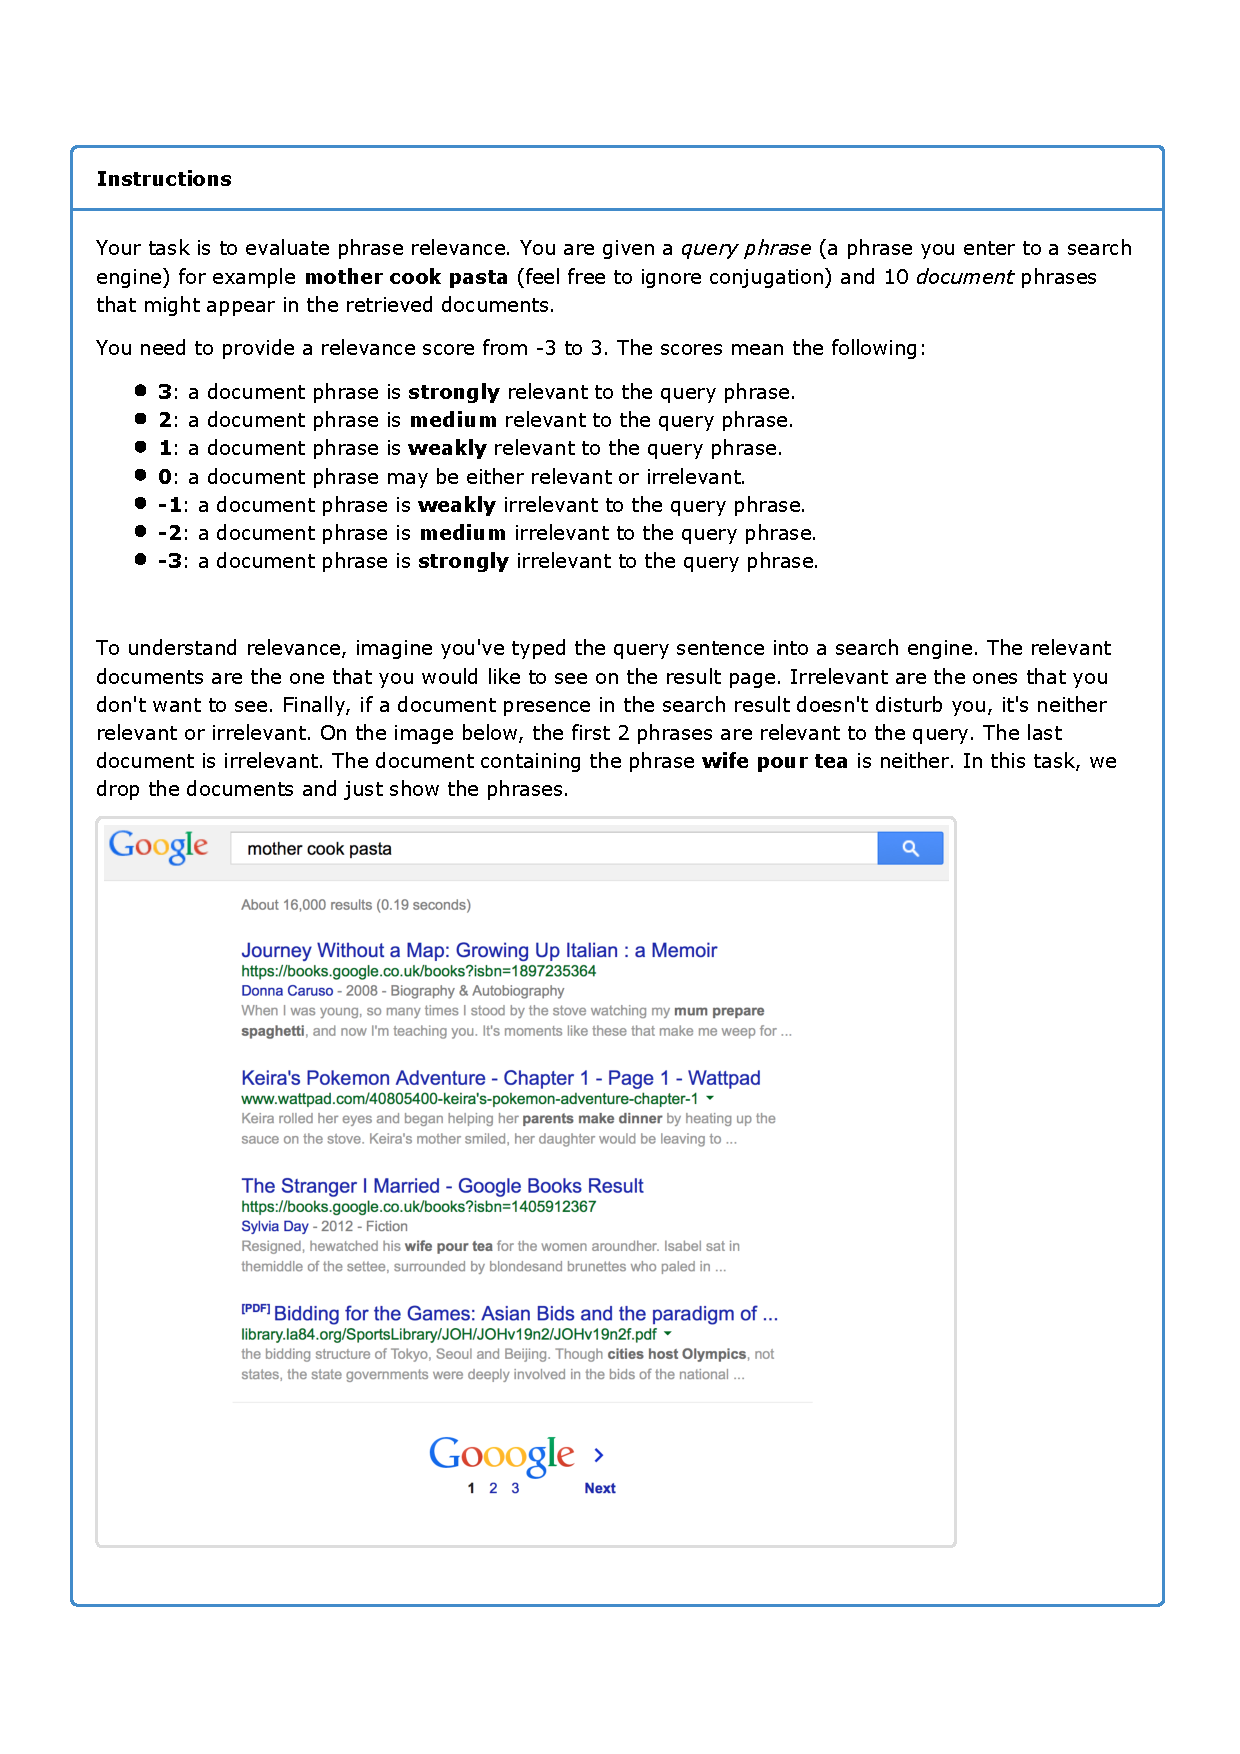
\includegraphics[width=0.9\textwidth]{figures/instructions}

\caption{Instructions given to the Mechanical Turkers}

\label{fig:instructions}
\end{figure}

%%% Local Variables:
%%% mode: latex
%%% TeX-master: "../paper.tex"
%%% End:


We recruited 19 human subjects using the Amazon Mechanical Turk platform.\footnote{\url{https://requester.mturk.com/}} Before answering a question, the subjects were given the instructions shown in Figure~\ref{fig:instructions}.

Each query-document pair was judged by three different people. The data was collected in two batches. Each question (or a HIT, Human Intelligence Task, in the Mechanical Turk terminology) consisted of a query phrase and 20 document sentences for the first batch and 10 documents for the second batch. Documents were shuffled before being shown to a human subject. Each document had to be judged for relevance using the following scoring system:
\begin{compactitem}
\item \textbf{-3}: strong irrelevance,
\item \textbf{-2}: medium irrelevance,
\item \textbf{-1}: weak irrelevance,
\item  \textbf{0}: a document may be either relevant or irrelevant,
\item  \textbf{1}: weak relevance,
\item  \textbf{2}: medium relevance,
\item  \textbf{3}: strong relevance.
\end{compactitem}

An example question is shown in Figure~\ref{fig:task}. The \dataurl{phraserel-raw.csv} file consists of human judgements together with anonymized Worker and HIT identifiers.

\begin{figure}
\centering
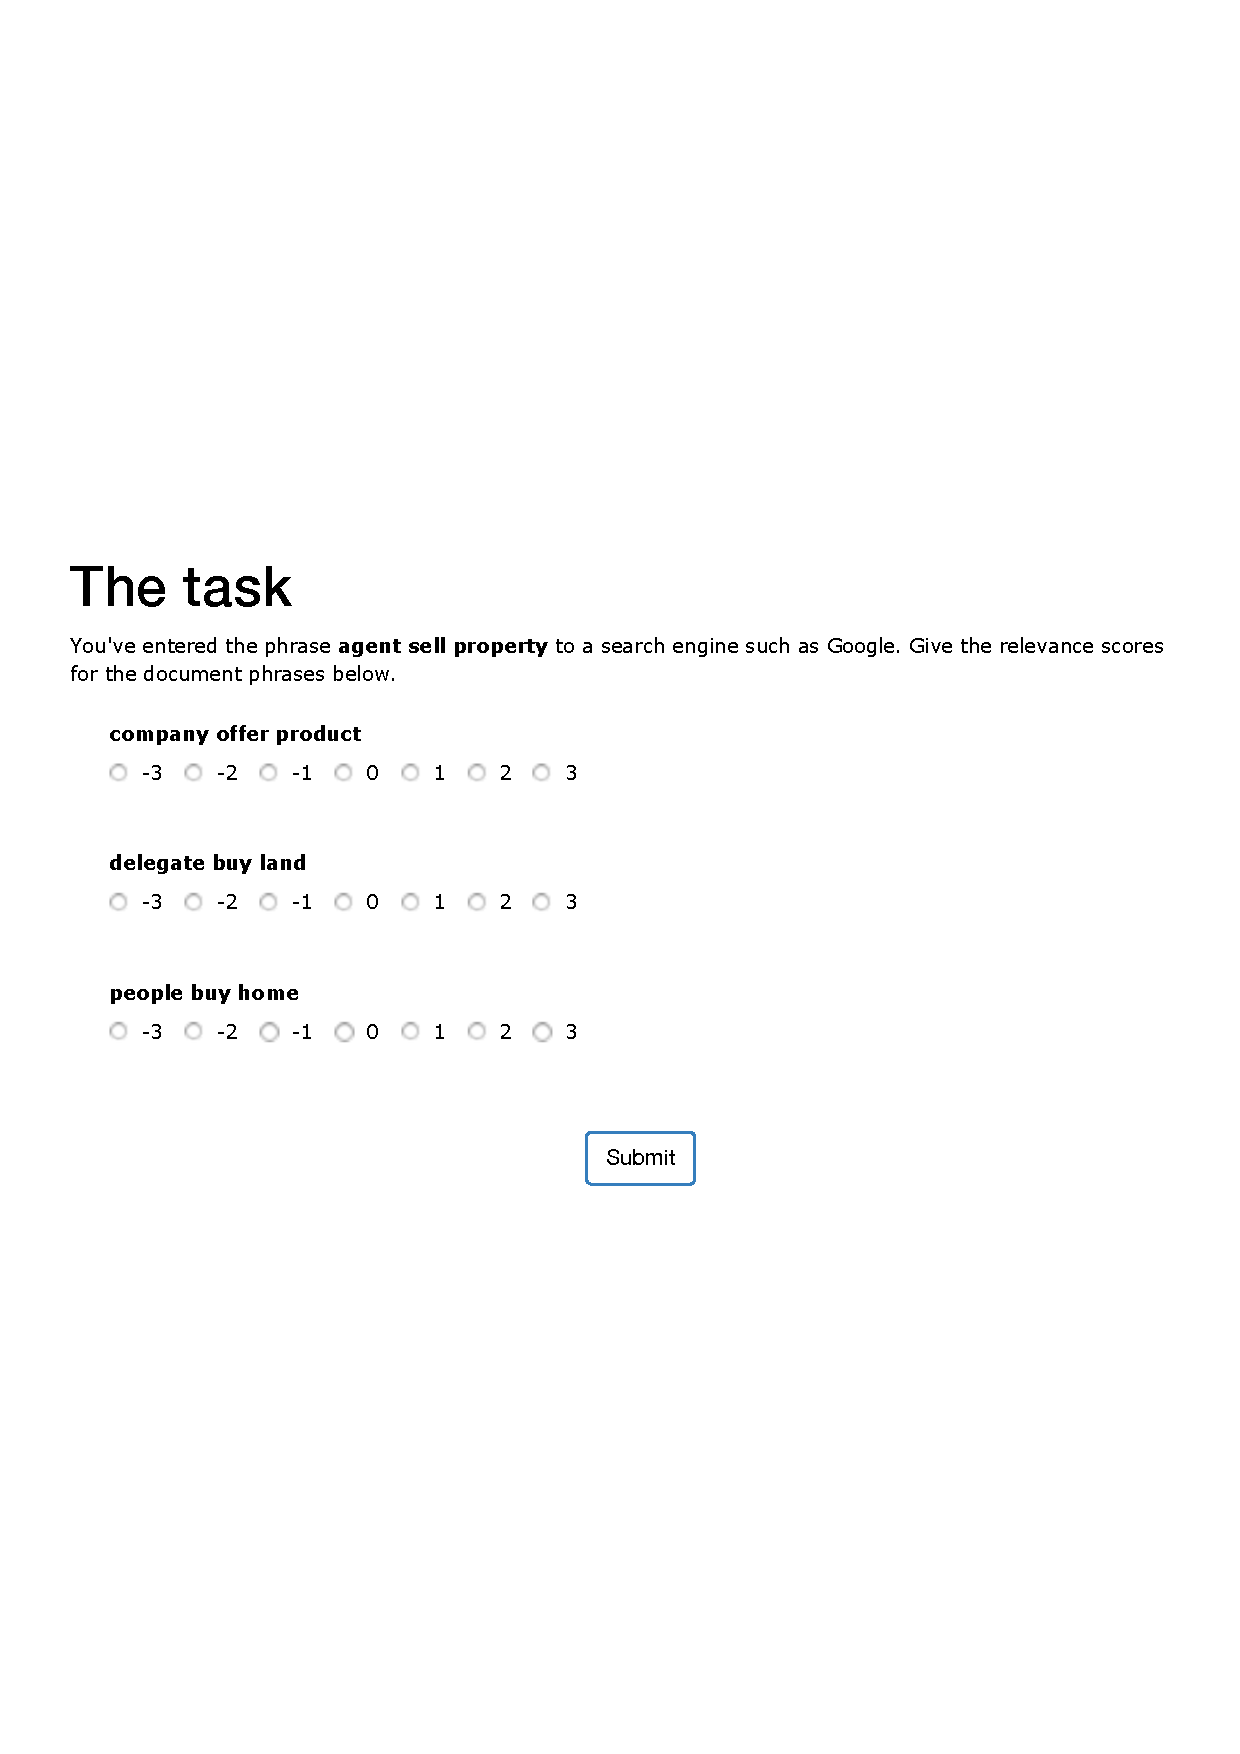
\includegraphics[width=0.9\textwidth]{figures/task}

\caption{\textbf{A sample question.}}

\label{fig:task}
\end{figure}

%%% Local Variables:
%%% mode: latex
%%% TeX-master: "../paper.tex"
%%% End:


\section{Final dataset construction}
\label{sec:postprocessing}

\subsection{Pair classification}

The pairs have been classified by the individual relevance judgements. A pair is of the \textit{strict relevance} type if all human judgements are greater than or equal to 0 and there is at least one 3 (strong relevance). A pair of the \textit{loosely   relevant} type is a pair where all human judgements are greater than or equal to 0. Figure~\ref{fig:emnlp-pairing} shows the mean and standard deviation of human judgements per query-document pair and the relevance division of a pair if applicable. There are 110 (or 7\%) strictly relevant pairs and 221 (13\%) loosely relevant pairs.
% * <sdyck@ualberta.ca> 2016-11-04T13:35:55.761Z:
%
% >  greater than or equal to 0
%
% but no 3's? otherwise loosely and strictly relevant classifications would overlap (all strictly would also be loosely) if that makes sense. 
%
% ^.

\subsection{Query classification}

Each query has been classified by the number of strictly relevant documents it has been paired with. On average, each query in the dataset is paired with 3.3 loosely relevant and 1.6 strictly relevant documents. The minimum number of loosely relevant documents per query is 1, the maximum is 14. Regarding the strict relevance, there are 8 queries without a single strictly relevant document, and the maximum number of strictly relevant documents per query is 7.

A query is \textit{diverse} if it is paired with 4 or more loosely relevant documents. There are 28 (42\%) such queries. On average, diverse queries are paired with 5.2 loosely relevant documents and 2.4 strictly relevant documents.
% \begin{compactitem}
% \item 14 queries with 4 loosely relevant documents,
% \item 6 with 5,
% \item 5 with 6,
% \item 1 with 7,
% \item 1 with 9,
% \item 1 with 14.
% \end{compactitem}

%%% Local Variables:
%%% mode: latex visual-line
%%% TeX-master: "thesis"
%%% TeX-engine: xetex
%%% End:
